\documentclass{instrukcja}        
\usepackage[polish]{babel}
\usepackage{amsmath}
\usepackage[utf8]{inputenc}
\usepackage[OT4]{fontenc}

\begin{document}
\materialnumber{4}
\course[Info I]{Informatyka I}
\material[Lab 4+]{Instrukcja 4+}
\author{B. Górecki}
\materialtitle


\section{Wskaźniki i referencje - bezboleśnie}
Nauczyliśmy się do tej pory, że funkcje w języku C mogą zwracać wartość. Co jednak, gdybyśmy chcieli napisać funkcję, która rozwiąże równanie kwadratowe i zwróci jego dwa rozwiązania? Jest to niemożliwe z użyciem tego mechanizmu - funkcja może zwrócić bowiem jedną i tylko jedną wartość! Do zwrócenia dwóch wyników potrzebujemy innego mechanizmu. Nie możemy tego zrobić z użyciem wartości zwracanej przez funkcję. Wyobraźmy sobie następujący kod funkcji {\tt main}.
\begin{verbatim}
void main()
{
   double a, b, c, x1, x2;
   a = 1;
   b = -3;
   c = 2;

   RozwiazRownanieKwadratowe(a, b, c, ...inne argumenty...);

   printf("x1 = %lf, x2 = %lf\n", x1, x2);
}
\end{verbatim}
Powyżej zależałoby nam na tym, aby funkcja {\tt RozwiazRownanieKwadratowe} była w stanie ,,w jakiś sposób'' wpisać rozwiązanie do zmiennych {\tt a} i {\tt b} zadeklarowanych wewnątrz funkcji {\tt main()}. Taki mechanizm zapewniają w języku C wskaźniki.

\section{Wskaźniki - trochę istotnej teorii}
W pewnym uproszczeniu pamięć operacyjną komputera (w której przechowywana jest każda ze zmiennych, jakie deklarujemy w kodzie - de facto wartość tej zmiennej) można postrzegać jako zbiór komórek. To tak zwany liniowy model pamięci. Każda z tych komórek może przechowywać jedną wartość. Każda ma też swój adres (komputer musi się do nich jakoś odnosić). Adresy przedstawione są jako liczby w formacie szesnastkowym (patrz Rys. 1). 
\begin{figure}[h!]
\centering
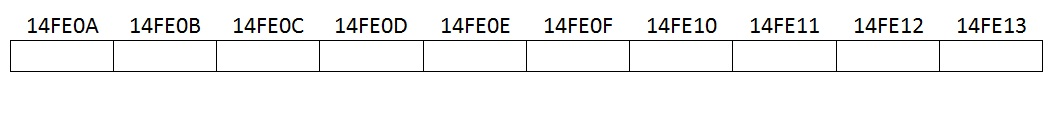
\includegraphics[width=0.45\textwidth]{pamiec1.jpg}
\caption{Liniowy model pamięci}
\end{figure}
Mając na uwadze taki model pamięci, prześledźmy następujący kod.
\begin{verbatim}
void main()
{
   int a;
}
\end{verbatim}
W tym momencie dokonaliśmy deklaracji zmiennej {\tt a}, tzn. zarezerwowana została dla niej jakaś komórka w pamięci komputera. Podczas pisania tej instrukcji, mój komputer zarezerwował dla zmiennej {\tt a} komórkę o adresie 14FE0F. Obecny stan obrazuje Rys. 2. Zacienienie oznacza, że zadeklarowaliśmy zmienną i to miejsce zostało zarezerwowane właśnie dla niej. Pod komórką (w celach czysto dydaktycznych) podpisaliśmy, jaka zmienna jest przechowywana w danej komórce pamięci.
\begin{figure}[h!]
\centering
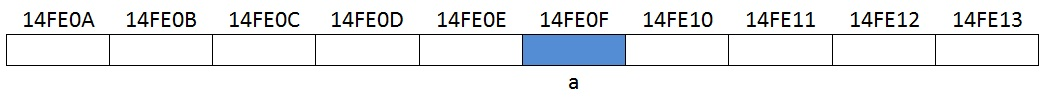
\includegraphics[width=0.45\textwidth]{pamiec2.jpg}
\caption{Zadeklarowana zmienna w pamięci}
\end{figure}

Teraz dokonamy przypisania wartości do zmiennej {\tt a}.
\begin{verbatim}
void main()
{
   int a;
   a = 5;
}
\end{verbatim}
Obecną sytuację obrazuje Rys. 3.
\begin{figure}[h!]
\centering
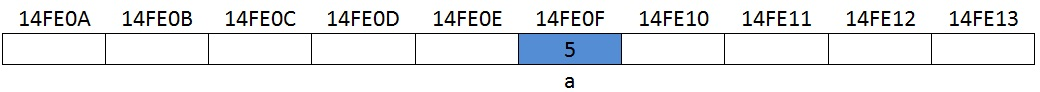
\includegraphics[width=0.45\textwidth]{pamiec3.jpg}
\caption{Zadeklarowana zmienna w pamięci oraz przypisana do niej wartość}
\end{figure}

Wydrukujmy teraz na ekran adres komórki, w jakiej przechowywana jest zmienna {\tt a} oraz samą wartość tam przechowywaną (czyli de facto wartość zmiennej {\tt a}). Operatorem wyłuskania adresu jest operator {\tt \&}. Aby więc uzyskać adres zmiennej {\tt a}, trzeba napisać {\tt \&a}. Przepisz poniższy kod, który ilustruje powyższy opis.
\begin{verbatim}
void main()
{
   int a;
   a = 5;
   printf("Adres komorki to %X, a wartosc to %d.\n", &a, a);
}
\end{verbatim}
Powyższa sekwencja formatująca {\tt \%X} nie różni się niczym od standardowego {\tt \%d} poza tym, że wydrukuje liczbę w notacji szesnastkowej, a nie dziesiętnej. Powinieneś na ekranie zobaczyć wynik zbliżony do poniższego.
\begin{verbatim}
Adres komorki to 14FE0F, a wartosc to 5.
\end{verbatim}
\subsection*{Dalej o wskaźnikach i referencjach}
Wróćmy teraz do naszego przykładu funkcji obliczającej pierwiastki równania kwadratowego i mającej ,,w jakiś sposób'' zwrócić do funkcji {\tt main} dwa rozwiązania. Wiemy, że wykorzystywana przez nas wcześniej instrukcja {\tt return} zwraca wartość jako wynik działania funkcji. To ważne! Zwraca wartość, a nie jakąś zmienną. To tak (upraszczając), jakby w jakimś biurze siedziała pani wykonująca te same zadania, co nasza funkcja, a wynik (wartość) zwracała nam jako liczbę zapisaną na kartce. Oczywiście dostajemy więc samą liczbę i nie wiemy nic o tym, co ta pani policzyła (lub jakich wzorów użyła i jakimi literkami sobie oznaczyła poszczególne wielkości). My (w funkcji {\tt main}) następnie bierzemy tę kartkę i zapisaną na niej liczbę wpisujemy w jakieś miejsce w pamięci. Tyle w funkcji {\tt main} oznacza taki kawałek kodu:
\begin{verbatim}
c = Suma(a, b);
\end{verbatim}
Chcemy jednak zwrócić dwie wartości. W powyższy sposób nie da się tego zrealizować w języku C (pani nie zna żadnego mechanizmu wydania nam dwóch kartek). Ale gdyby udało nam się powiedzieć tej pani, że gdy już się w swoim biurze doliczy dwóch wyników, to zamiast cokolwiek zapisywać na kartce (i oddawać nam) ma po prostu kartkę z jednym wynikiem zanieść do domu stojącego pod jednym adresem (czyli wpisać jakąś wartość do zmiennej w pamięci komputera), a kartkę z drugim wynikiem zanieść do domu stojącego pod drugim adresem, to po zakończeniu działania funkcji (mimo, że funkcja nie zwróciła przez wartość zwracaną żadnego wyniku) mielibyśmy oba wyniki wpisane w odpowiednich miejscach w pamięci. Przejdźmy do formalizmu języka C. Napiszmy funkcję {\tt DodajOdejmij}, która przyjmie dwie wartości typu {\tt double}, obliczy sumę i różnicę tych liczb i nie zwróci żadnego wyniku przez wartość zwracaną, ale wpisze zarówno sumę, jak i różnicę bezpośrednio w odpowiednie miejsca w pamięci. Zgodnie z powyższą historyjką, musi w tym celu znać też adresy tych zmiennych. Przyjmie je również na liście argumentów. Przepisz poniższy kod funkcji.
\begin{verbatim}
void DodajOdejmij(double a, double b, double &suma, double &roznica)
{
   suma = a + b;
   roznica = a - b;
}
\end{verbatim}
Na liście argumentów poinformaliśmy znakiem {\tt \&} kompilator o tym, że funkcja przyjmie adresy, a wewnątrz ciała funkcji możemy już używać zmiennych {\tt suma} i {\tt roznica} jako normalnych zmiennych. Dopiszmy jeszcze kod funkcji {\tt main}.
\begin{verbatim}
void main()
{
   double a = 12;
   double b = 10;
   double suma, roznica;

   DodajOdejmij(a, b, suma, roznica);

   printf("Suma = %lf, Roznica = %lf\n", suma, roznica);
}
\end{verbatim}
Właśnie zwróciliśmy z funkcji dwie wartości przez referencję (czyli tak naprawdę adres). Przyjrzyjmy się jeszcze wskaźnikom. Wróćmy w tym celu do naszego liniowego modelu pamięci komputera. Wskaźnik to taka zmienna, która wskazuje miejsce w pamięci, w którym przechowywana jest inna zmienna. Możemy na przykład pokazywać na zmienną {\tt a}. Wskaźnik (zmienną typu wskaźnikowego) deklarujemy przez poprzedzenie jej nazwy znakiem {\tt *}. Przyjrzyjmy się przykładowi.
\begin{verbatim}
void main()
{
   int a;
   a = 5;
   int *p;
}
\end{verbatim}
W tym momencie {\tt a} jest zadeklarowane jak poprzednio, zaś {\tt p} to zmienna, która ma na coś pokazywać. Niemniej to też zwykła zmienna, więc zarezerwowano dla niej jakieś miejsce w pamięci (Rys. 4).
\begin{figure}[h!]
\centering
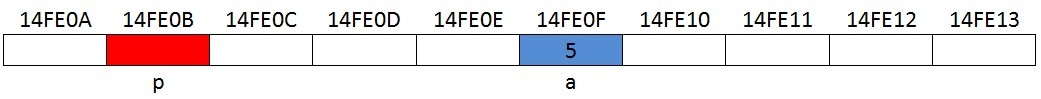
\includegraphics[width=0.45\textwidth]{pamiec4.jpg}
\caption{Zadeklarowana zmienna p oraz a (na razie nic o sobie nie wiedzą)}
\end{figure}

Zmienna {\tt p} jednak na razie na nic nie pokazuje. Jest dokładnie taką samą zmienną, jak każda inna. Trzeba jej więc przypisać, na co ma pokazywać. Chcemy, aby pokazywała na zmienną {\tt a}. Pokazywać to znaczy nic innego niż znać adres, gdzie przechowywana jest zmienna {\tt a}. Wtedy każdemu, komu wskaźnik {\tt p} ma wskazać zmienną {\tt a} mówi po prostu, gdzie ona ,,mieszka''. Dokonajmy więc tego przypisania. {\tt p} musi przechowywać adres zmiennej {\tt a}.
\begin{verbatim}
void main()
{
   int a;
   a = 5;
   int *p;
   p = &a;
}
\end{verbatim}
Dopiero teraz stworzyliśmy powiązanie! {\tt p} pokazuje na {\tt a} (Rys. 5).
\begin{figure}[h!]
\centering
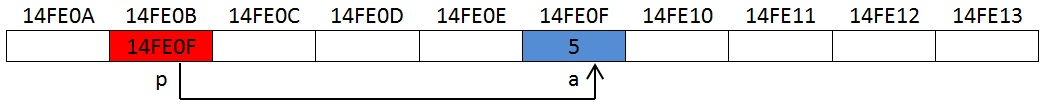
\includegraphics[width=0.45\textwidth]{pamiec5.jpg}
\caption{Zadeklarowana zmienna {\tt p} (wskaźnik), który teraz już pokazuje na zmienną {\tt a} (zna po prostu jej adres - tzn. wartość przechowywana w zmiennej {\tt p} to adres zmiennej {\tt a})}
\end{figure}

\subsection*{Zapamiętaj!}
Zmienna {\tt p} przechowuje adres {\tt a}. Natomiast używając zapisu {\tt *p} możesz wyłuskać wartość, na jaką {\tt p} pokazuje. Czyli my wyłuskamy wartość przechowywaną w zmiennej {\tt a}.

Przepisz teraz kod, który zobrazuje to, czego dokonaliśmy.
\begin{verbatim}
void main()
{
   int a;
   a = 5;
   int *p;
   p = &a;
   
   printf("Wartosc a = %d, adres a = %X\n", a, &a);
   printf("Wartosc p = %X, wartosc pokazywana przez p = %d\n", p, *p);
}
\end{verbatim}
Skompiluj i uruchom program. Powinienes uzyskać napis zbliżony do poniższego.
\begin{verbatim}
Wartosc a = 5, adres a = 14FE0F
Wartosc p = 14FE0F, wartosc pokazywana przez p = 5
\end{verbatim}

Przepisz jeszcze poniższy program i samodzielnie (wstawiając w odpowiednich miejscach instrukcje {\tt printf} drukujące wartość zmiennej {\tt a}) przeanalizuj, jak działa.
\begin{verbatim}
void main()
{
   int a;
   int *p;
   p = &a;

   *p = 8; // wpisujemy 8 w miejsce pokazywane przez p
         // Jaka jest teraz wartosc a?

   a = 10; // Jaka jest teraz wartosc wskazywana przez p?
}
\end{verbatim}

\section{Zwracanie wartości przez wskaźnik}
Wcześniej napisaliśmy funkcję, która zwraca dwie wartości przez referencję. Można tego samego dokonać przez wskaźnik. Analogiczny kod funkcji {\tt DodajOdejmij} ma następującą składnię (teraz zamiast referencji na liście argumentów przekazujemy wskaźniki).
\begin{verbatim}
void DodajOdejmij(double a, double b, double *suma, double *roznica)
{
   *suma = a + b;
   *roznica = a - b;
}
\end{verbatim}
Pamiętaj, że w przypadku użycia wskaźników wewnątrz funkcji musisz używać cały czas operatora {\tt *}, aby przypisać coś do wartości wskazywanej przez wskaźnik. Kod funkcji {\tt main} jest teraz taki:
\begin{verbatim}
void main()
{
   double a = 12;
   double b = 10;
   double suma, roznica;

   // Deklarujemy wskazniki
   double *WskaznikNaSuma, *WskaznikNaRoznica;

   // Dokonujemy przypisania do zmiennych, na ktore maja pokazywac
   WskaznikNaSuma = &suma;
   WskaznikNaRoznica = &roznica;

   DodajOdejmij(a, b, WskaznikNaSuma, WskaznikNaRoznica);

   printf("Suma = %lf, Roznica = %lf\n", suma, roznica);
}
\end{verbatim}

Zauważmy jeszcze na koniec, że jawne deklarowanie wskaźników na sumę i różnicę oraz jawne powiązywanie ich z sumą i różnicą jest zbędne. Możemy tego dokonać wprost przy wywołaniu funkcji (na liście jej argumentów), bowiem tylko do funkcji muszą trafić odpowiednio powiązane wskaźniki, a de facto adresy (bo właśnie adresy wskaźniki przechowują). Gdy dokonamy tego uproszczenia, funkcja {\tt main} ma następującą formę. Przeanalizuj bardzo dokładnie, na czym polega uproszczenie.
\begin{verbatim}
void main()
{
   double a = 12;
   double b = 10;
   double suma, roznica;

   DodajOdejmij(a, b, &suma, &roznica);

   printf("Suma = %lf, Roznica = %lf\n", suma, roznica);
}
\end{verbatim}

\subsection*{Ćwiczenia}
Napisz funkcję, która rozwiąże równanie kwadratowe (przy danych współczynnikach {\tt a, b, c}) i zwróci oba rozwiązania. Napisz dwa warianty tej funkcji - jeden, który dokona tego przez referencję; drugi - który dokona tego przez wskaźniki. Odpowiednio dostosuj funkcję {\tt main} do każdego z wariantów.
\subsection*{Zapamiętaj!}
Do poprzednich zajęć wszystkie nasze funkcje przyjmowały argumenty jako wartości (tworzone były dla nich lokalne kopie samych wartości przechowywanych w zmiennych) i również zwracały wartości (a nie zmienne). Tym samym funkcje mogły zmieniać swoje lokalne kopie pewnych zmiennych, ale nie wpływało to na wartości tych zmiennych poza tą funkcją. Natomiast za każdym razem, gdy używasz wskaźnika, bądź referencji, działasz na rzeczywistym miejscu w pamięci, w którym ta zmienna jest przechowywana. Tzn. że tak dokonane modyfikacje będą widziane na zewnątrz funkcji po jej wykonaniu. Obrazuje to poniższy przykład. Po każdym wywołaniu dowolnej funkcji dopisz instrukcję, która wydrukuje ci na ekran wartość zmiennej {\tt a} i {\tt b}.
\begin{verbatim}
void fun1(int a)
{
   a = 2 * a;
}

void fun2(int &a)
{
   a = a + 3;
}

int fun3(int a)
{
   return 3 * a;
}

void fun4(int *a)
{
   *a = 8;
}

void main()
{
   int a = 5;

   fun1(a);
   // Wydrukuj tu wartosc a
   fun2(a);
   fun3(a);
   a = fun3(a);
   fun4(&a);
   fun2(a);
}
\end{verbatim}
Poćwicz jeszcze samodzielnie, aby nabrać przekonania i pewności, że rozumiesz ten mechanizm.

\end{document}
